
\label{sect:compensation}

Para realizar la compensación de Miller del amplificador, y determinar el valor del capacitor, es necesario relevar la ganancia de lazo con la frecuencia. Teóricamente para realizar una compensación por polo dominante con un margen de fase de $45 \si[per-mode=symbol]{\degree}$, debería colocarse el polo, de tal forma de que la ganancia de lazo sea de exactamente $0 \si[per-mode=symbol]{\decibel}$, donde se encuentre el primer polo natural del circuito. La técnica usada prácticamente es observar en forma aproximada donde se localiza este punto y con un valor aproximado de la resistencia a frecuencias medias \quotemarks{vista} por el capacitor de Miller, determinada por inspección, tener una primera aproximación de la frecuencia del polo, usando el $\tau_{RC}$ calculado aproximadamente, luego el valor se refina por prueba y error, para finalmente llevar el valor óptimo a un valor comercial. El circuito utilizado para relevar la ganancia de lazo se puede observar en la figura~\figref{fig:fig_circuit_compensation}, en el mismo se introduce la señal de prueba a través de la entrada inversora del amplificador diferencial con un capacitor de acople de alto valor, luego de haber pasivado la señal de entrada, se introduce un resistor de \quotemarks{separación}, que permite observar la señal en la salida del amplificador, luego de haber pasado por la red de realimentación y el amplificador, obteniéndose de esta forma la ganancia de lazo. Se pretende mantener el punto de reposo inalterado, para lograr esto, se altera también el resistor colocado en la otra entrada del amplificador diferencial, de manera de compensar el offset que se produce por la caída provocada por las corrientes de base de los transistores del par diferencial.\\

El valor determinado aproximadamente, está en el orden de las decenas de $\si[per-mode=symbol]{\pico\farad}$, por lo tanto se partió de un valor de $100 \si[per-mode=symbol]{\pico\farad}$, el cual se fue bajando hasta lograr la compensación buscada. \\

El valor comercial seleccionado finalmente para el capacitor de compensación es de  $39 \si[per-mode=symbol]{\pico\farad}$. En la figura~\figref{fig:fig_loop_gain} se puede observar el gráfico de la ganancia de lazo en magnitud y fase resultante, el mismo se realizó en \textbf{MATLAB} con datos exportados desde \textbf{LTSPICE}, para mayor claridad. \\

Algo importante a observar, es que se observa un par de polos complejos conjugados alrededor de los $25 \si[per-mode=symbol]{\mega\hertz}$, este par de polos introducen un giro de fase extra de $90 \si[per-mode=symbol]{\degree}$, además del sobre-pico en la ganancia, llevando al amplificador mas cerca de la inestabilidad a esta frecuencia. Es posible que en este caso, a pesar de haberse logrado una compensación correcta a $45 \si[per-mode=symbol]{\degree}$, sea conveniente llevar ese margen a un valor un poco mayor. Estos polos que se observan parecen ser introducidos por los transistores usados en el VAS, \textbf{MPSA42} y \textbf{MPSA92}, no se observa al reemplazar los mismos con otros transistores, podría ser una peculiaridad de los transistores o de los modelos (proveídos por el fabricante).

\clearpage

\begin{figure}[H] %htb
\begin{center}
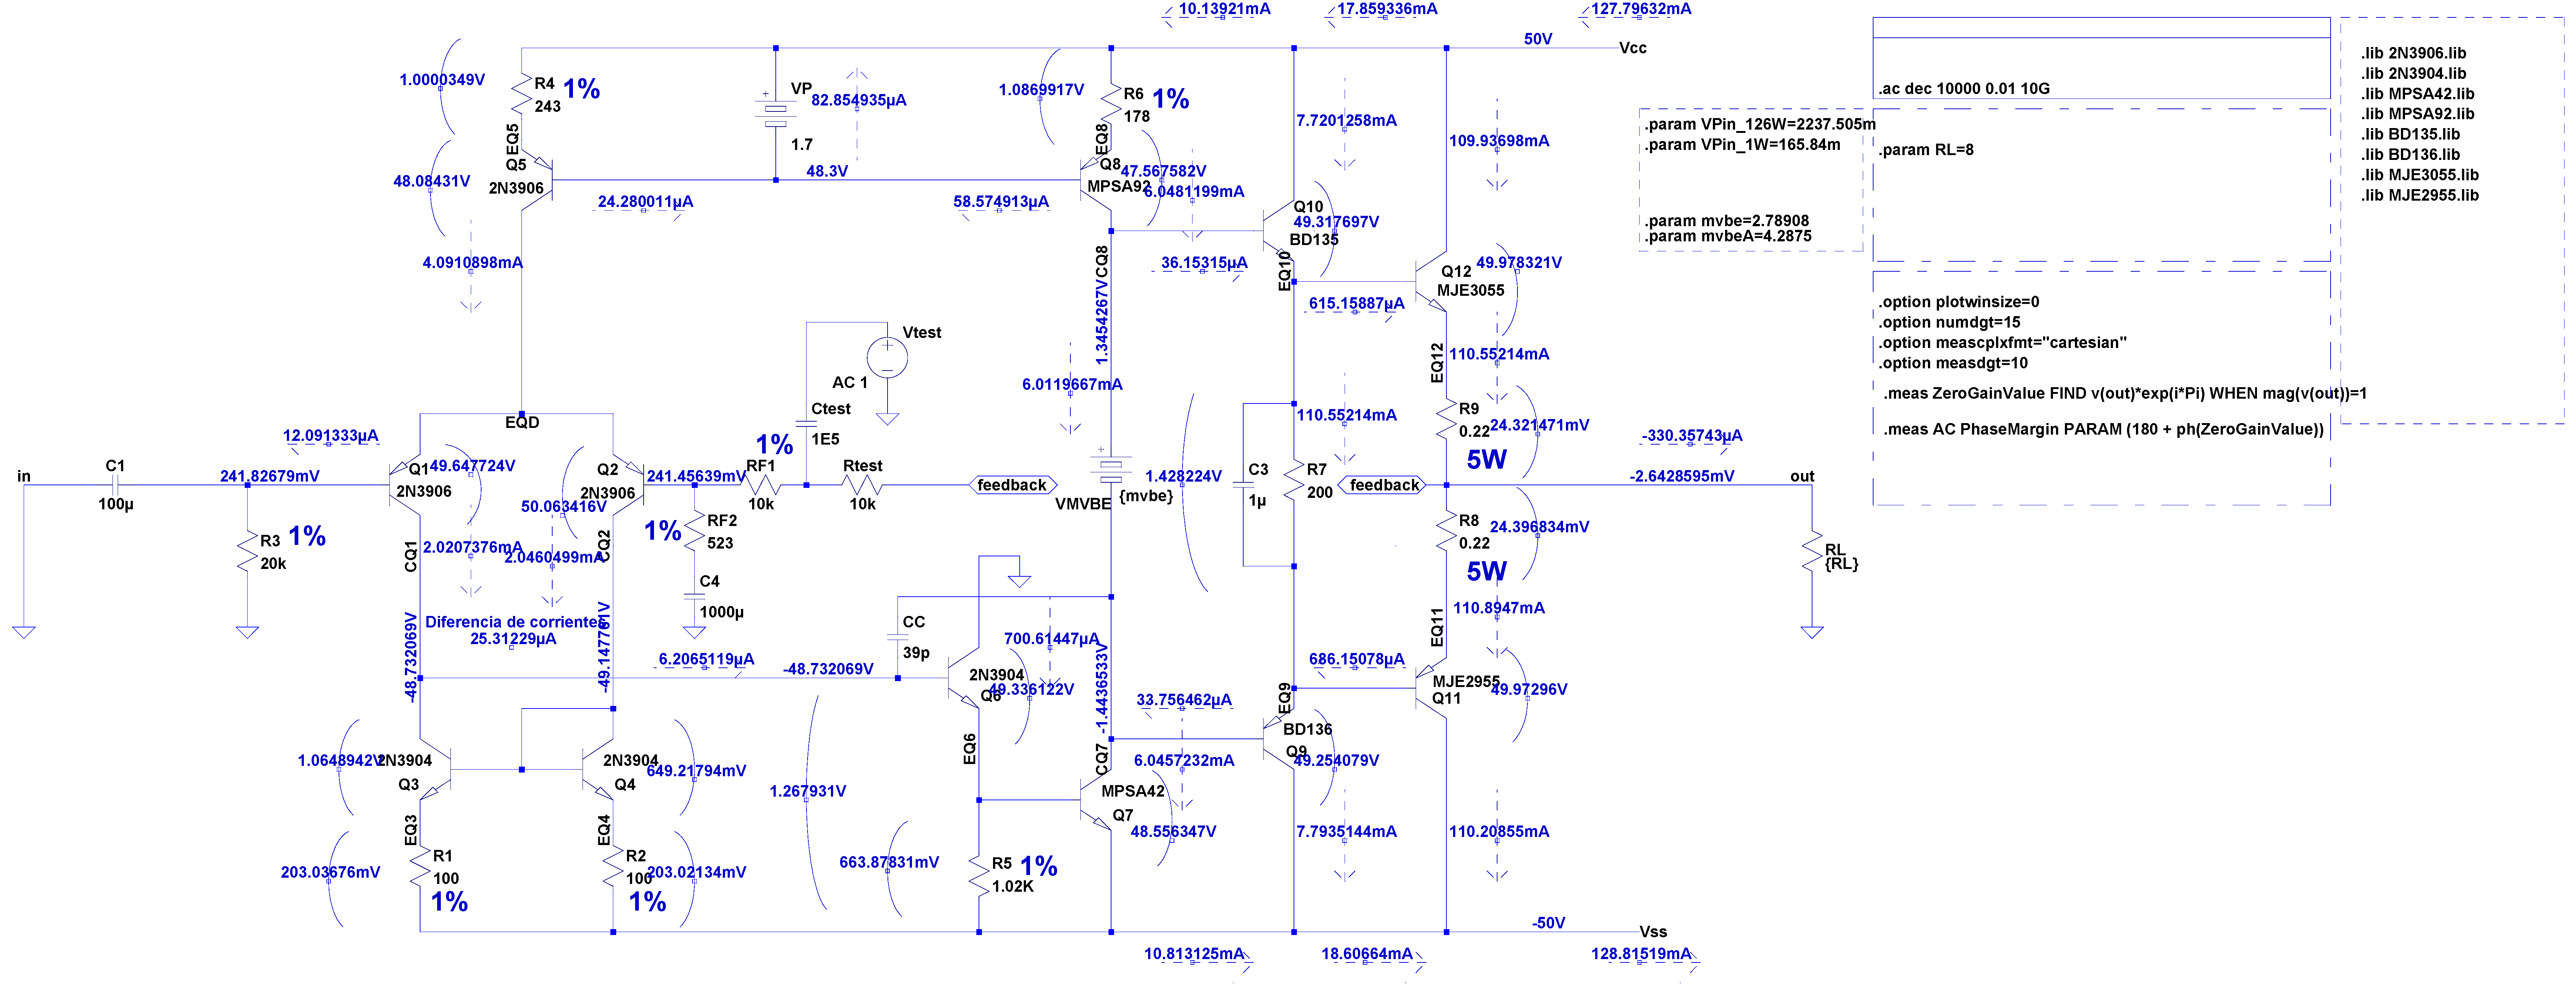
\includegraphics[width=0.93 \textheight, angle=90]{./img/circuits/amplifier_LOOP.png}
\caption{\label{fig:fig_circuit_compensation}\footnotesize{Circuito usado para determinar la ganancia de lazo.}}
\end{center}
\end{figure}

\clearpage

\begin{figure}[H] %htb
\begin{center}
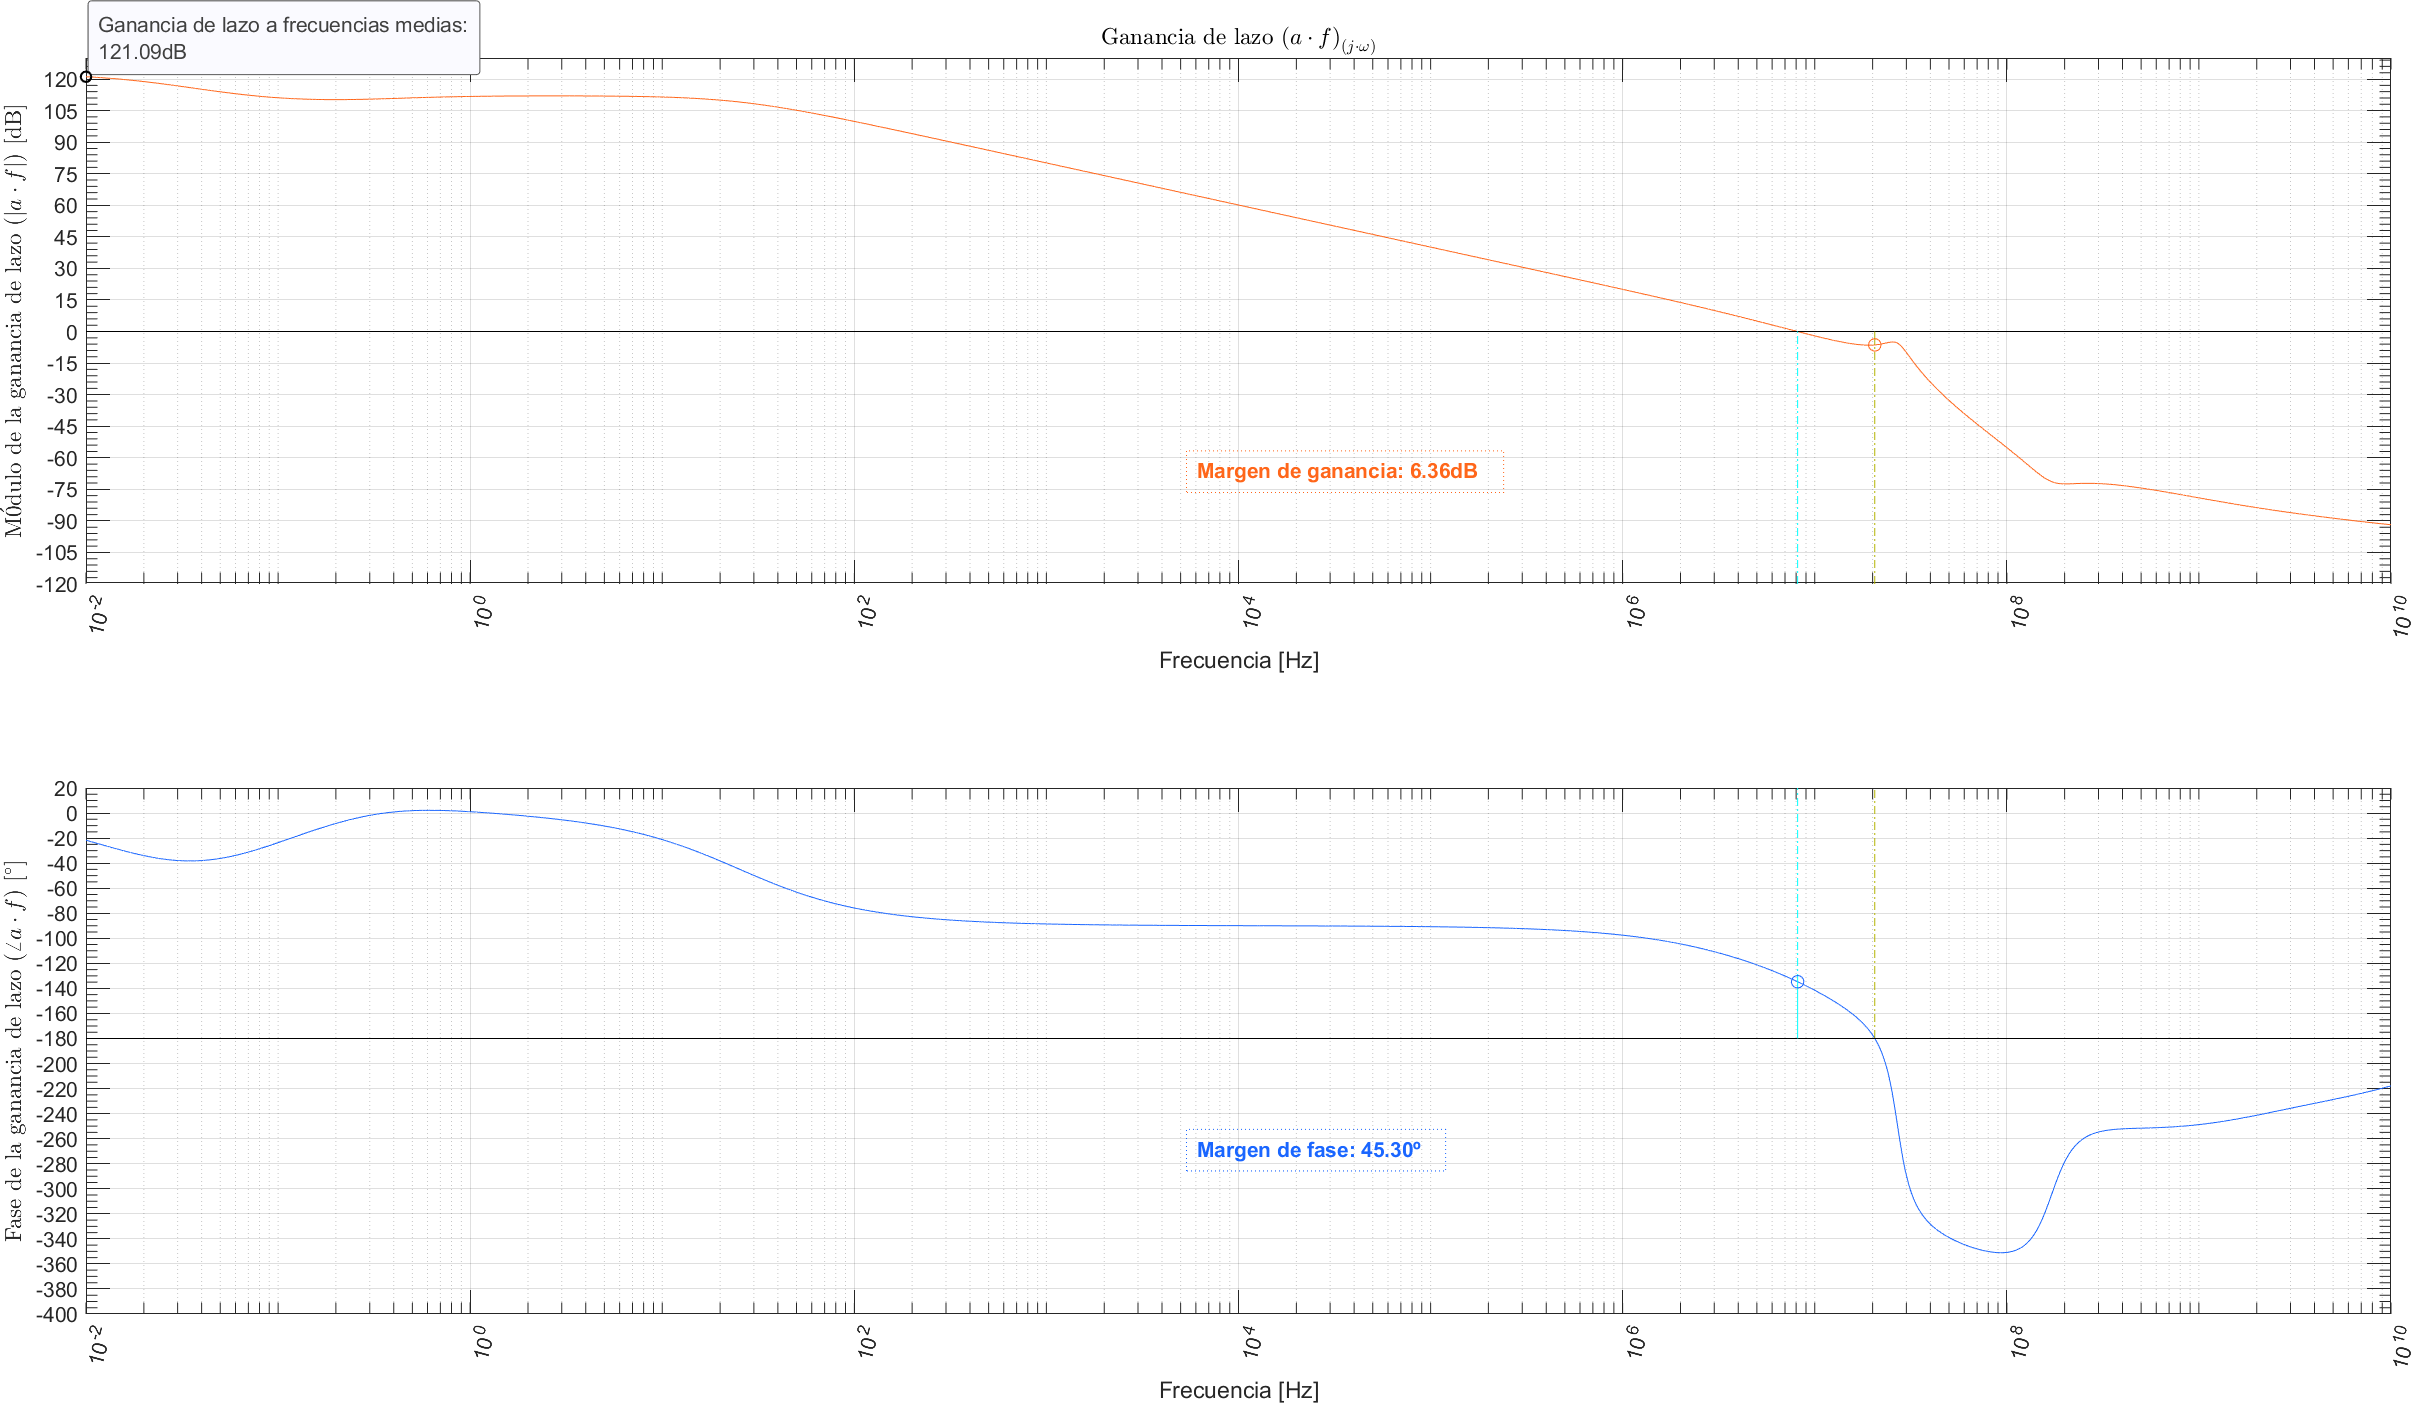
\includegraphics[width=0.93 \textheight, angle=90]{./img/simulaciones/Loop/gain_loop.png}
\caption{\label{fig:fig_loop_gain}\footnotesize{Ganancia de lazo en función de la frecuencia, indicando los márgenes obtenidos.}}
\end{center}
\end{figure}

\clearpage